\chapter{Introduction}
\label{chapter:intro}

The modern economy revolves around stock market.
Stock market is a way for companies to obtain capital which they can invest into their own business.
In exchange, the person who invests into the companies stocks technically owns a piece of the company which can return profit to the investor two different ways.
The stock can grow in value, which allows the investor to sell the stock in higher price or the company itself can pay dividends to investors based on the number of stocks the investor owns from the company.

The price of the stock is simply determined by the law of supply and demand. 
If somebody is willing to pay a higher price for the stock then the price of the stock can grow.
Because of this the stock market is in continuous fluctuation where people are selling and buying the stocks with the price they think the stock is worth using stockbrokers as the middleman. \cite{person}
All of this has lead to the question, how can we invest most optimally into stocks?
This is where the following computational methods come in. 

There are many strategies on how to invest into these stocks which depend on multiple factors such as; how much do you expect to profit with your investment, how much are you willing to take risk, do you want to make money by selling the stocks or by receiving dividends and so on.
The underlying principle with every strategy is to minimize the risk you need to take in order to gain as much as profit as possible.
Some of the strategies are based on subjective evaluation of the companies, but more technical strategies use metrics that are calculated from the financial statistics or the real-time market values.
Strategies using the former data are called fundamental analysis and the strategies using latter data technical analysis.
Neither of these approaches can predict the future of the market, but can statistically decrease the probability of larger losses in the market for the investor altough the probability of large losses is still not zero with these methods. \cite{fox}

Fundamental analysis is based on the idea that each stock has a intrinsic value that can be larger than the actual price of the stock in the market and buying these will eventually lead to profits.\cite{sohnke}
The fundamental analysis focuses on the financial metrics that consist of companys overall statistics.
These are for example how much the company has made profit, how much the company has paid dividends and what is companys cash flow.
These tell a lot about the growth of the company and how the future of the company looks like.
These metrics are usually published quarterly four times a year and present more long-term statistics about the company.
Because of this, the amount of data these values present is quite small in terms of space.

The technical analysis that focuses on the real-time market values, on the other hand, needs new data almost daily.
Stock exchanges are usually open from morning, opening around 8 to 10am, until evening, closing around 5 to 7pm on weekdays.
Before and after this there are more limited pre- and after-hours trading which lasts usually around 1 to 2 hours depending on the exchange in which more limited stock trades can be made.
During these hours multiple values are recorded on the prices of the stock from which the most important ones being: the highest price the stock was sold, the highest price the stock was sold and the number of stocks traded during the time interval.
The technical analysis focuses on finding recognizable patterns through this data. \cite{murphy}
Where the data used by the fundamental analysis was relatively small, these values can generate gigabytes of raw data in a week.

Developing a system that can be used to conduct technical analysis means that the system should be planned to be able to handle large amounts of these data as time progresses.
As such task is not trivial, the goal of this thesis is to provide developers and researchers, who want to analyse this data efficiently, basic knowledge and tools on what are the best current solutions on handling this data.
With this knowledge these data scientists can save considerable amount of time without the need of trial and error when developing this kind of system from the ground up.

% for screenshots
\begin{figure}[ht]
    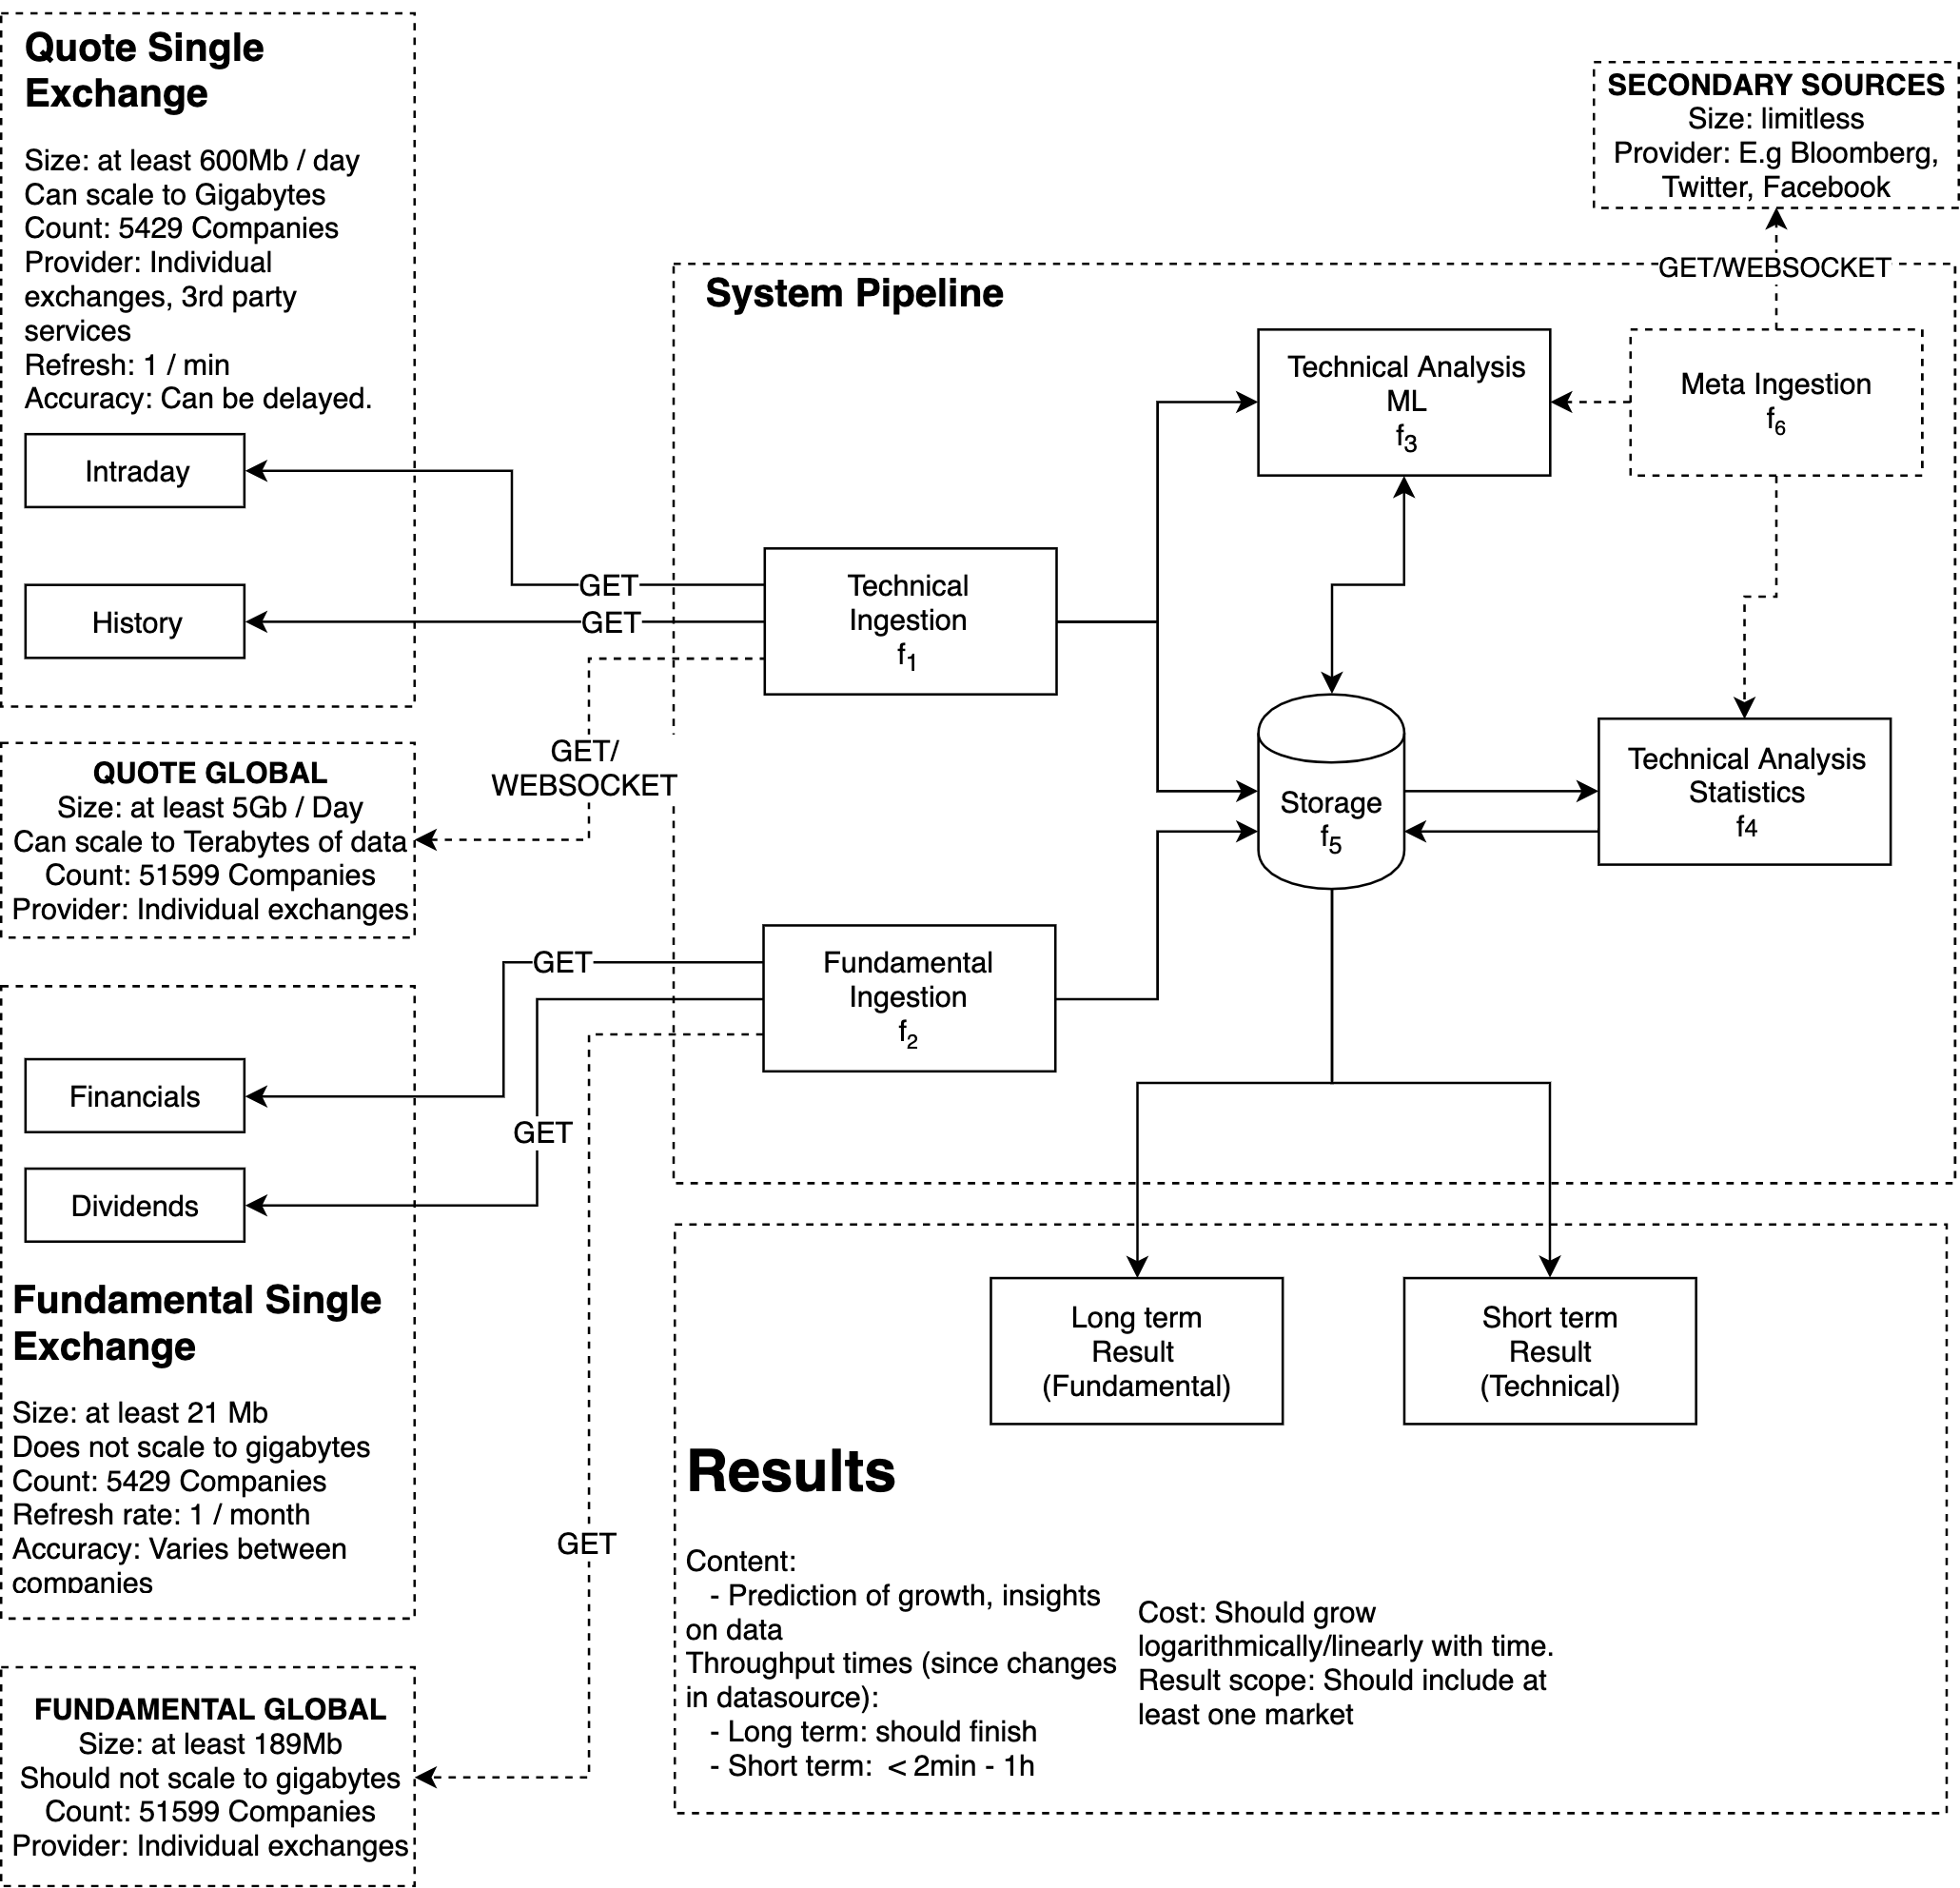
\includegraphics[scale=0.36]{images/system2} 
    \centering
    \caption{Example of a stock data pipeline}
\end{figure}

\section{Application scenario}
% research and engineering questions (why do you have to do it and why it is new)

To have a better picture what are the challenges of developing a system for technical analysis are, we will next look at a example case.
This is to give reader more practical and meaningful view on the problem at hand.

Somewhat normal system for analysing both fundamental and technical analysis is presented in figure 1.
In the figure, the components marked with solid lines represent the core system functions, and the dashed lines represent add-on functionalities that should be possible to extend into the system in the future.
The requirements of the system should be as follows;
The system should produce long ($r_1$) and short ($r_2$) term predictions of stock prices.
The computation of long term predictions can take time because of the nature of these predictions but the short term predictions should be between two minutes to one hour available.
Long term predictions are the result of fundamental analysis ($f_2$) and historical technical analysis ($f_4$) whereas the short term prediction should come mostly from quick technical analysis ($f_3$).
The cost of the system should grow logarithmically/linear with time meaning that the cost of processing and storing data should not exponentially increase over time.
Finally, the core system should be able to fulfill these requirements for at least the +5000 companies in the major U.S stock markets.

The data to the application is ingested from two main types of data sources quote and fundamental.
These sources consist of values that were briefly described previously in technical and fundamental analysis respectively.
The quote data is usually updated with minute intervals depending on the provider whereas the fundamental data does not change so often.
Theoretically, the fundamental data can change anytime, because of dividends which can be payed whenever the companies want but this does not happen often and these values are mostly used in the long term fundamental analysis so longer update intervals are acceptable.
In the figure, these are separated into the U.S market ones ($d_1$ and $d_2$) and the other sources ($d_3$ and $d_4$) that provide the same data on other global markets.
The extendable global data sources are grouped into one box but in reality this data would be ingested from numberable different providers as there is no single entity at the time of writing this that provides all of this data.
Theoretically the maximum size of this extendable data would be 5Gb per day which is extrapolated in from the U.S market data based on statistics that in January 2019 there were globally 51 599 companies listed in the stock markets \cite{global}.
This amount can and will fluctuate as companies enter and exit the markets but it gives us the scale of data we are working with.

Today, stock market analysis has also a large focus on predicting stock prices using secondary data sources that can have reflect and affect the prices of stocks. 
These secondary data sources can be anything but at the moment one of the most researched sources are traditional media and social media data.
Examples of using this kind of data to predict predict stocks can be found in \cite{kao}, \cite{skuza} and \cite{wai}.
This is why the system should have the ability to extend to ingest data from arbitrary secondary sources ($f_6$ and $d_5$ in the figure) to provide more versatile predictions about the stocks.
The amount of this data can be unlimited but is restricted to relevant sources.

Data is ingested from these data sources mainly using HTTP-protocol as this is the main method that these services ($d_1$ - $d_4$) provide.
Other possible methods that are usually available are Excel sheets and sometimes websockets, of which the websockets can be actually useful in cloud system, but as the HTTP-methods are currently the most used technology, this thesis is also going to focus on these.
Here we have separated the main ingestion functions into two main types of functions $f_1$ and $f_2$. 
$f_1$ is constantly polling and processing data whereas $f_2$ handles batch processing.
Both of these function store their raw output into the storage, but $f_1$ passes this also to the immediate technical analysis.

The system has two technical analysis functions.
For methdos that allow streaming updates there is $f_3$, which can for example be cumulative/reinforced ML models and for methods that need historical data in order to calculate the prediction, there is $f_4$.
For fundamental analysis, there is no a specific function as the introduced data sources usually provide these values pre-calculated and these values are usually easy to calculate dynamically with little to none amount of processing.

Finally, at the center of the system is the storage which is used to store the calculated predictions as well as the raw data from the data sources for later analysis.
For historical technical analysis, $f_4$, the storage should provide reasonable range query times when quering historical data and for the results the storage should provide efficient point queries for the results ($<$ 1s).

\section{Research Questions}

The focus of this thesis is going to be the part of the pipeline that calculates predictions based on historical data.
This means the ingestion, storage and analysis of this data.
As we have seen in the previous section, the system has to have the ability to grow, and we are going to focus on how to implement this in practice.

As the field of possible technologies is large, the main focus of this thesis would be the comparison of current relevant technologies in the context of stock data to help data scientists to decide what technologies to possibly use in their own projects.
The main result of this thesis would be information and possible tools that developers could use to develop this kind of system more efficiently.
Developers here can be people from companies that either do stock analysis as their main business or just want to analyze stock data efficiently.
These results could also be used in research to implement analyzing pipelines more efficiently so that the research group can focus on the analyzing of the stock data instead of worrying with getting the data to these parts.

Analyzing the stock data is also what most of the research today is focused on as this is the part that can actually produce profit.
This means that most papers ignore the steps of ingesting and storing this data.
Examples of this kind of papers are \cite{wu}, \cite{aghakhani} and \cite{kao}.
So one of the goals of this thesis would be to bring more comprehensive picture on stock data pipelines. 

This thesis will approach this subject from three different perpectives that cumulate on one another.
These perspectives are represented by the following three research questions:

What are the needs and requirements of this kind of system data-wise?
What are the methods currently used to conduct technical analysis and possibly what kind of data they use.
This thesis plans to provide the information on these so that when a reader is developing their own system they have a point of reference which they can use to evaluate their data sources.

What are technological options to implement a modern scalable timeseries analysis pipeline?
As there are enormous amount of different technological frameworks, this thesis plans to provide the reader information on the most promising ones currently.
This way the reader does not need to go through and learn variety of technologies in order to build their system.

How to implement big data framework for technical analysis in practice?
Finally the thesis plans to provide comparison and prototype implementations of stock data ingestion using the technologies that seem most prominent.
The metrics used to compare these systems would be the response time, possible scalability and the time it takes to develop these systems.
This is to save possible time of a person developing these when the trial and error is done beforehand and if the prototype system fits the developed architecture it can also be used as a basis for further development by the reader.

\section{Expected Outcome}

For the first research question "What are the needs and requirements of this kind of system data-wise?" this thesis plans to provide an analysis of the necessary stock market data and its usages.
From this analysis, the thesis would derive the main requirements for the system to fulfill in order to satisfy the needs of the possible subsequent analysis stage.
This result could then be used in the future if one would want to build their own ingestion system from the ground up as a base.

For the second question "What are technological options to implement this in practice?" the thesis would perform an analysis on the current trends in data ingestion solutions.
The thesis would provide information on the latest open-source technologies that could be used to implement this kind of system, how these would fulfill the requirements introduced by the first research question with application scenario and conclude this with a comparison of these technologies on what are the advantages of using one over another.
The result of this part could be used to decide what seems to be the most suitable technology to use to implement the application scenario technically. 

For the last question "How do the most viable big data ingestion options compare to one another in the context of stock data perfomance-wise?" the thesis would implement open-source prototype solutions based on the results of the second research question.
This prototype could be used by anybody (company or individual) as it is or as a base to build a more complex system on top of it.
The system would be targeted to practically implement the described application scenario, which could be used by companies with similar products allowing them to write more complex analysis algorithms based on the larger amount of data.

\section{Structure of the Thesis}

In the first chapter of the thesis we will be focusing on solving the first research question "What are the needs and requirements of this kind of system data-wise?".
The thesis would start by going through scientific papers about stock markets and stock analysis.
There would be first text generally about the characterics of the stock markets, what are they based on, what affects them, can they actually be predicted (random walk hypothesis) and so on.
Then the thesis would go through the main directions of analysing the stock markets (fundamental analysis, technical analysis) and explain briefly some of the methods (about three methods per direction) that characterize these directions (Gordon model, Magic formula, LSTM etc.) focusing on the data that these methods need in order to calculate their predictions.
This part would be concluded by deriving the requirements for the system based partly on these analysis methods and their data needs, and partly on the definitions that make up a scalable, secure and stable cloud system.
The next step would be solving the second research questions "What are technological options to implement this in practice?".
This step would perform literary research on what is currently used to perform big-data ingestion and storing, selecting from the list of technologies mostly those that seem to fulfill the requirements derived in the step 1 and would fit in the application scenario introduced in figure 1, specifically in $f_1$ and $f_2$.
For data ingestion, these technologies would probably be Apache NIFI, Apache Flume, Fluentd etc. 
For data storage, these could be HDFS, HDFS, Apache HBase, Apache Cassandra etc.
This step would consist of first introducing all of the selected technologies and going through how do they work, what are they supposed to solve and what are the advantages and disadvantages of using one.
After this, the section would do a comparison of these technologies in the context of stock data and conclude with analysis on which of the technologies would be the most prominent ones to solve this problem.
After this would start the experimental part of the thesis and the rest of thesis would be focusing on solving the final research question "How do the most viable big data ingestion options compare to one another in the context of stock data perfomance-wise?".
Based on the results of the step 2, I would implement couple of the most prominent solutions as a prototype systems.
This step would include the actual implementations and reporting of these implementations.
The report would consist of technical details; what parts does each of the system consists of, what versions were used, where the system was run etc. And subjective remarks; was it easy to implement, was there parts that did not fit together etc. 
The reporting part would also explain the metrics that would be measured for the subsequent analysis.
For these metrics, the dataset used to test the system would be the open-source REST API from IEX \cite{iex}, which is open for consumers until first of June, 2019.
These metrics could be, for example, the time it takes to batch process, processor usage, memory usage, database fetching times etc. 
As these systems would be run inside Docker containers, the tools used to measure these metrics would most probably be programming language specific functions and Docker specific statistics tools. 
In the final step, the thesis would first inspect the results from the step 3 and based on these make remarks on what could be the best potentially the best implementation in this context.
After this there would be an wrap-up on each of the previous sections concluding in retrospective what could've been possibly done better and what could be done in the future, concluding in recommendation what could be based on this thesis the best technical solution to implement system described in the application scenario. 
